\section{Experiments} \label{sec:experiments}

This section presents an extensive experimental evaluation of PASS. We present the datasets, implementation details, and results over several LNL benchmarks, followed by an ablation study.

\begin{table}[t!]
    \centering
    \caption{Test accuracy (\%) on CIFAR-100~\cite{krizhevsky2009learning} subject to various IDN noise rates~\cite{xia2020part}. The results were obtained from~\cite{Garg_2023_WACV}, wherein the base model (\(*\)) results are denoted in \textit{italics}. \(\dagger\) represents the SOTA and \textbf{PASS} represents our approach with mentioned baselines.}
    \label{tab:cifar}
    \begin{tabular}{l c c c c c}
        \toprule
        \textbf{Method} & \textbf{0.20} & \textbf{0.30} & \textbf{0.40} & \textbf{0.45} & \textbf{0.50} \\
        \midrule
        CE~\cite{yao2021instance}  & 30.42 & 24.15 & 21.45 & 15.23 & 14.42\\
        %CausalNL~\cite{yao2021instance}  & 41.47 & 40.98 & 34.02 & 33.34 & 32.13\\
        USDNL~\cite{xu2023usdnl} & 64.82 & 61.35 & 55.82 & - & 46.00 \\
        PTD-R-V~\cite{xia2020part}  & 65.33 & 64.56\ & 59.73 & - & 56.80 \\
        % Co-teaching~\cite{han2018co}  & 37.96 & 33.43 & 28.04 & 25.60 & 23.97 \\
        MentorNet~\cite{jiang2018mentornet}  & 38.91 & 34.23 & 31.89 & 27.53 & 24.15\\
        % kMEIDTM~\cite{cheng2022instance}  & 69.16 & 66.76 & 63.46 & - & 59.18\\
        \midrule
        DivideMix*~\cite{li2020dividemix}  & \textit{77.07} & \textit{76.33} & \textit{70.80} & \textit{57.78}  & \textit{58.61}\\
        \rowcolor{Gray!25} \textbf{DivideMix-PASS}  & \textbf{77.41} & \textbf{76.58} & \textbf{75.07} & \textbf{72.91}  & \textbf{72.27}\\
        \midrule
        InstanceGM*~\cite{Garg_2023_WACV}  & \textit{79.69} & \textit{79.21} & \textit{78.47} & \textit{77.49}  & \textit{77.19}\\
        % \rowcolor{Gray!25} \textbf{InstanceGM-PASS}  & \textbf{81.02} & \textbf{80.33} & \textbf{79.28} & \textbf{78.69}  & \textbf{78.26}\\
        \rowcolor{Gray!25} \textbf{InstanceGM-PASS} & \withdagger{\textbf{81.02}} & \withdagger{\textbf{80.33}} & \withdagger{\textbf{79.28}} & \withdagger{\textbf{78.69}} & \withdagger{\textbf{78.26}}\\
        \bottomrule
    \end{tabular}
\end{table} 

\subsection{Datasets}\label{subsec:dataset}

The experiments are performed on many common datasets in LNL, including CIFAR-100~\cite{krizhevsky2009learning}, CIFAR-N~\cite{wei2022learning}, Animal-10N~\cite{song2019selfie}, Red mini-ImageNet~\cite{jiang2020beyond}, Clothing-1M~\cite{xiao2015learning} and mini-WebVision~\cite{li2020dividemix}.
%CIFAR10/100
\paragraph{CIFAR-100} The dataset consists of \(50,000\) training images and \(10,000\) testing images with each image having a size of \(32 \times 32 \times 3\) pixels, distributed evenly into 100 categories. This dataset does not possess label noise by default, so we follow the \emph{part-dependent label noise} setting~\cite{xia2020part} to simulate various IDN noise rates: \(\{0.2, 0.3, 0.4, 0.45, 0.5\}.\)

%CIFARN
\paragraph{CIFAR-10N and CIFAR-100N} The datasets are created by relabelling both the original CIFAR-10 and CIFAR-100~\cite{wei2022learning} datasets using the Amazon Mechanical Turk (M-Turk) labelling service.
%which involves annotations from human workers. 
The CIFAR-10N dataset includes five distinct noise rate options, from which we have selected the \say{\emph{worst}} version (noise rate of \(40.21\)\%). In the CIFAR-100N dataset, we considered \say{\emph{fine}} labels with an overall noise level of \(40.20\)\%.

%Animal-10N
\paragraph{Animal-10N} This is a real-world dataset including \(10\) animal categories, with \(5\) pairs of animals sharing similar appearances, such as \emph{chimpanzee} and \emph{orangutan}. The dataset has an estimated label noise rate of \(8\%\), and it comprises of \(50,000\) training images and \(10,000\) test images. In the experiments, we do not perform data augmentation to be consistent with the standard setup~\cite{song2019selfie} for a fair evaluation.
 
 %Redmini-ImageNet
\paragraph{Red mini-ImageNet} The dataset is a subset of the real-world CNWL dataset, which is mainly established to examine the impact of label noise rates on image classification. This dataset includes 100 categories where each categories consists of \(600\) colour images. To ensure an equitable comparison to previous studies, all images have been resized to 32\(\times\)32 pixel\({}^{2}\). There are various noise rates ranging from \(0\% \text{ to } 80\%\). We focused on the noise rates of \(40\%, 60\%, \text{ and } 80\%\) to maintain consistency with the existing literature~\cite{Garg_2023_WACV, xu2021faster}.
% \begin{figure}[t!]
    \centering
    \begin{tikzpicture}
        \pgfplotstableread[col sep=comma, header=true]{smoothed_loss_data.txt} \myTable
        \begin{axis}[
            height=0.37\linewidth,
            width=0.85\linewidth,
            xlabel={Number of epochs},
            xlabel style={font=\footnotesize},
            xticklabel style={font=\footnotesize},
            ylabel={Loss Values},
            ylabel style={font=\footnotesize, yshift=-0.5em},
            yticklabel style={font=\footnotesize},
            xmin=30, xmax=302, % Adjust x-axis limits as per your data
            legend style={draw=none, font=\footnotesize, yshift=-2em, /tikz/every even column/.append style={column sep=1em}},
            legend columns=2,
            scale only axis
        ]
            \addlegendentry{DivideMix-PASS (Ours)};
            \addplot[mark=*, mark size=1.5pt, mark repeat=0, mark phase=0, MidnightBlue!70, thick, solid] table[x={Epoch}, y={TotalLoss}]{\myTable};

            % \addlegendentry{Labeled Loss (Your Approach)};
            % \addplot[mark=square*, mark size=1.5pt, BurntOrange!70, thick, solid] table[x={Epoch}, y={LabeledLoss}]{\myTable};
            
            \addlegendentry{DivideMix};
            \addplot[mark=square, mark size=1.5pt, ForestGreen!70, thick, solid] table[x={Epoch}, y={DM_TotalLoss}]{\myTable};

            % \addlegendentry{DM Labeled Loss};
            % \addplot[mark=triangle*, mark size=1.5pt, Red!70, thick, solid] table[x={Epoch}, y={DM_UnlabeledLoss}]{\myTable};
        \end{axis}
    \end{tikzpicture}
    \caption{Comparison of training loss over epochs between DivideMix-PASS (ours) and DivideMix~\cite{li2020dividemix} on CIFAR-100~\cite{krizhevsky2009learning} at \(0.5\) IDN~\cite{xia2020part}. 
    \gustavo{Why do we need this figure?}
    %\textcolor{MidnightBlue}{\textbf{--}} represents DivideMix-PASS, \textcolor{ForestGreen}{\textbf{- -}} indicates DivideMix~\cite{li2020dividemix}.
    }
    \label{fig:lossComparison}
\end{figure}
%Clothing1M
\paragraph{Clothing1M} This is also a real-world dataset consisting of 1 million training images collected from \(14\) distinct online shopping website categories. There is an estimated \(38.5\%\) noise level in this dataset's labels, which are derived from the surrounding text. To ensure comparability, we used downsized images to \(256 \times 256\) pixel\(^{2}\), as per the prevalent format in previous works~\cite{Garg_2023_WACV, li2020dividemix}. There are \(50,000, 14,000, \text{ and } 10,000\) manually authenticated training, validation, and testing samples, respectively. We excluded clean training and validation sets during training. We only use the clean test set for evaluation, following the literature~\cite{Garg_2023_WACV, li2020dividemix}.


\begin{table}[t!]
    \centering
    \caption{Test accuracy (\%) on CIFAR-N~\cite{wei2022learning}, where results of other models are from~\cite{wei2022learning}. The \textbf{PASS} base model  is DivideMix~\cite{li2020dividemix} (\(*\) with results in \textit{italics}) and \(\dagger\) represents the SOTA.}
    \label{table:cifar100N}
    \begin{tabular}{l c c}
        \toprule
        \bfseries Method & \bfseries CIFAR10N-W & \bfseries CIFAR100N-F  \\
        \midrule
        CE~\cite{liu2022robust} & 77.69 & 55.50\\
        CAL~\cite{zhu2021clusterability} & 85.36 & 61.73\\
        ELR~\cite{liu2020early} & 91.09 & 66.72\\
        % SOP+~\cite{liu2022robust} & 93.24 & 67.81\\
        %ProMix  & \textbf{96.16} & \textbf{73.39}\\
        \midrule
        DivideMix*~\cite{li2020dividemix} & \textit{92.56} & \textit{71.13}\\
        \rowcolor{Gray!25} \textbf{DivideMix-PASS}  & \withdagger{\textbf{94.02}} & \withdagger{\textbf{72.03}} \\
        \bottomrule
    \end{tabular}
\end{table}
\begin{table}[t]
        \centering
        \caption{Test accuracy (\%) of various approaches on Animal-10N~\cite{song2019selfie} with baseline (\(*\) and outcomes in \textit{italics}). The other results are  from~\cite{feng2021ssr}. \textbf{PASS} represents our approach with baseline DivideMix~\cite{li2020dividemix} and SSR~\cite{feng2021ssr}, and \(\dagger\) denotes the SOTA.}
        \label{table:Animal10N}
        \begin{tabular}{l c}
            \toprule
            \bfseries Method & \bfseries Test Accuracy (\%) \\
            \midrule
            CE~\cite{zhang2021learning} & 79.4 \\
            SELFIE~\cite{song2019selfie} & 81.8 \\
            PLC~\cite{zhang2021learning} & 83.4 \\
            % Nested-CE~\cite{chen2021boosting} & 84.1 \\
            Jigsaw-ViT~\cite{chen2023jigsaw} & \textbf{89.0}\\
            \midrule
            DivideMix*~\cite{li2020dividemix} & \textit{81.40}\\
            \rowcolor{Gray!25}\textbf{DivideMix-PASS} & \textbf{82.90} \\
            \midrule
            SSR*~\cite{feng2021ssr} & \textit{88.5}\\
            \rowcolor{Gray!25} \textbf{SSR-PASS} & \withdagger{\textbf{89.2}} \\
            \bottomrule
        \end{tabular}
    \end{table}
% \input{main/train_label_unlabel}
%mini-Webvision
\paragraph{Mini-WebVision} The dataset consists of \(65,944\) colour images taken from the initial \(50\) categories of the WebVision dataset~\cite{li2017webvision}, with images reduced to \(256 \times 256\) pixels. In the experiments, we follow the standard benchmark by evaluating on the clean validation sets of both mini-WebVision and the equivalent \(50\) categories from the ImageNet dataset~\cite{deng2009imagenet}.


\subsection{Implementation}\label{subsec:implementation}

All methods are implemented in the PyTorch framework and executed on the NVIDIA RTX 3090 GPU computing platform. Baseline models are selected based on their accuracy and compatibility with the dataset under consideration. For CIFAR-100, the InstanceGM~\cite{Garg_2023_WACV} and DivideMix~\cite{li2020dividemix} models are used because both have demonstrated to be highly accurate. For CIFAR-N, the DivideMix~\cite{li2020dividemix} model is used. For Animal-10N, SSR~\cite{feng2021ssr} is selected as the base model. For Red mini-ImageNet, a hybrid approach using FaMUS~\cite{xu2021faster} with two evaluation versions, one with and one without DINO self-supervision~\cite{caron2021emerging} is employed. For Clothing-1M, AugDesc~\cite{nishi2021augmentation} model is used. For mini-WebVision, C2D~\cite{zheltonozhskii2022contrast} is employed as the base model. Unless otherwise stated, default hyperparameters and network architectures are as specified in their corresponding papers.

% \begin{table*}[htbp!]
%     \small
%     \centering
%     \caption{Test accuracy (\%) on (a) CIFAR-N~\cite{wei2022learning}, where results of other models are from~\cite{wei2022learning}. The \textbf{PASS} base model  is DivideMix~\cite{li2020dividemix} (\(*\) with results in \textit{italics}). (b) Test accuracy (\%) of various approaches on Animal-10N~\cite{song2019selfie} with baseline (\(*\) and outcomes in \textit{italics}) SSR~\cite{feng2021ssr}. The other results are  from~\cite{feng2021ssr}. \textbf{PASS} represents our approach with baseline SSR~\cite{feng2021ssr}.} \label{table:2}
%     \begin{subtable}[t]{0.5\linewidth}
%         \centering
%         \begin{tabular*}{\linewidth}{@{\extracolsep{0.5pt}}lcc}
%             \toprule
%             \textbf{CIFAR-N} & \small{\textbf{10N-W}} & \small{\textbf{100N-F}}  \\
%             \midrule
%             CE~\cite{liu2022robust} & 77.69 & 55.50\\
%             CAL~\cite{zhu2021clusterability} & 85.36 & 61.73\\
%             ELR~\cite{liu2020early} & 91.09 & 66.72\\
%             SOP+~\cite{liu2022robust} & 93.24 & 67.81\\
%             \midrule
%             DivideMix*~\cite{li2020dividemix} & \textit{92.56} & \textit{71.13}\\
%             \rowcolor{Gray!25} \textbf{DivideMix-PASS}  & \textbf{94.02} & \textbf{72.03} \\
%             \bottomrule
%         \end{tabular*}
%         \caption{CIFAR-N}\label{table:cifar100N}
%     \end{subtable}%
%     \hfill
%     \begin{subtable}[t]{0.45\linewidth}
%         \centering
%         \begin{tabular*}{\linewidth}{@{\extracolsep{0.5pt}}lc}
%             \toprule
%             \textbf{Animal-10N} & \textbf{Accuracy (\%)} \\
%             \midrule
%             CE~\cite{zhang2021learning} & 79.4 \\
%             SELFIE~\cite{song2019selfie} & 81.8 \\
%             PLC~\cite{zhang2021learning} & 83.4 \\
%             Nested-CE~\cite{chen2021boosting} & 84.1 \\
%             Jigsaw-ViT~\cite{chen2023jigsaw} & \textbf{89.0}\\
%             \midrule
%             SSR*~\cite{feng2021ssr} & \textit{88.5}\\
%             \rowcolor{Gray!25} \textbf{SSR-PASS} & \textbf{89.0} \\
%             \bottomrule
%         \end{tabular*}
%         \caption{Animal-10N}
%         \label{table:Animal10N}
%     \end{subtable}
% \end{table*}


\subsection{Comparisons on Benchmarks}\label{subsec:baseline}
In this section, we perform a comparison study on IDN benchmarks and real-world noisy-label benchmarks.

\subsubsection{IDN Benchmark}\label{subsubsec:idn_benchmark}
 
In \cref{tab:cifar}, a comparative analysis is presented showcasing the performance of the proposed method, PASS, against various SOTA techniques on the CIFAR-100 IDN benchmark~\cite{xia2020part}.
% In particular, PASS demonstrates significant improvements in this dataset across various IDN noise rates ranging from \(20\%\) to \(50\%\), when employing  InstanceGM~\cite{Garg_2023_WACV} and DivideMix~\cite{li2020dividemix} models as baselines. As baseline models represent the primary reference for PASS, it is critical to compare the performance of the postulated PASS method with these models to showcase the efficacy and adaptability of our work. Compared to current SOTA methods on this benchmark (InstanceGM~\cite{Garg_2023_WACV} and DivideMix~\cite{li2020dividemix}),
In particular, PASS outperforms these models by approximately between \(1.2\%\) to \(14\%\) at \(0.50\) noise rate. 
% We also provide the training loss over epochs in~\cref{fig:lossComparison}.\gustavo{can we remove this training loss from here? I'm not sure why we need it.}

\subsubsection{Real-world noisy-label benchmarks}\label{subsubsec:real-world}
In~\cref{table:cifar100N,table:Animal10N,table:RedMini,table:clothing1M,table:miniWebvision}, we showcase the results of our proposed method on CIFAR-N~\cite{wei2022learning}, Animal-10N~\cite{song2019selfie}, Red mini-ImageNet~\cite{jiang2020beyond}, Clothing1M~\cite{xiao2015learning}, mini-WebVision~\cite{li2020dividemix} and ImageNet~\cite{krizhevsky2012imagenet}. Overall, PASS demonstrates superior performance or competitiveness with current SOTA models.
% employing various baselines for both a large-scale web-crawled dataset and a small-scale human-annotated noisy dataset.
The results also show that PASS exhibits a high degree of flexibility and can be easily integrated into existing LNL models. 


\begin{table}[t!]
    \centering
    \caption{Test accuracy (\%) on Red mini-ImageNet (CNWL)~\cite{jiang2020beyond}. The additional results of the model are from~\cite{Garg_2023_WACV}. We show \textbf{PASS} (ours) using DivideMix~\cite{li2020dividemix} and FaMUS~\cite{xu2021faster} ($\ast$ and the results in \textit{italics}, \(\dagger\) represents the SOTA) without and with self-supervision (SS)~\cite{caron2021emerging}.}
    \label{table:RedMini}
    \begin{tabular}{l c c c}
        \toprule
        \multirow{2}{*}{\textbf{Red mini-ImageNet}} & \multicolumn{3}{c}{\textbf{Noise rate}} \\
        \cmidrule{2-4}
         & \textbf{0.4} & \textbf{0.6} & \textbf{0.8} \\
        \midrule
        CE~\cite{xu2021faster} &  42.70 & 37.30 & 29.76 \\
        % MixUp~\cite{zhang2017mixup} &  46.40 & 40.58 & 33.58 \\
        MentorMix~\cite{jiang2020beyond} &  47.14 & 43.80 & 33.46 \\
        InstanceGM~\cite{Garg_2023_WACV} &  52.24 & 47.96 & 39.62 \\
        \midrule
        DivideMix~\cite{li2020dividemix} & \textit{46.72} & \textit{43.14} & \textit{34.50} \\
        \rowcolor{Gray!25}\textbf{DivideMix-PASS}  & \textbf{53.02} & \textbf{48.01} & \textbf{38.62} \\
        \midrule
        FaMUS$\ast$~\cite{xu2021faster} & \textit{51.42} &  \textit{45.10} & \textit{35.50} \\
        \rowcolor{Gray!25}\textbf{FaMUS-PASS}  &  \withdagger{\textbf{53.40}} & \withdagger{\textbf{48.04}} & \withdagger{\textbf{40.08}} \\
        \midrule
        \multicolumn{4}{l}{\textbf{With self-supervised learning}} \\
        \midrule
        % PropMix~\cite{cordeiro2021propmix} & 56.22 & 52.84 & 43.42 \\
        InstanceGM-SS*~\cite{Garg_2023_WACV} & 56.37 & 53.21 & 44.03 \\
        \rowcolor{Gray!25}\textbf{FaMUS-SS-PASS}  & \withdagger{\textbf{56.48}} & \withdagger{\textbf{53.53}} & \withdagger{\textbf{44.32}} \\
        \bottomrule
    \end{tabular}
\end{table}

\begin{table}[t!]
    \centering
    \caption{Test accuracy (\%) of competing strategies on Clothing1M~\cite{xiao2015learning}. In the experiments, only noisy-labels are used for training. The base models used are DivideMix~\cite{li2020dividemix}, AugDesc~\cite{nishi2021augmentation} and FINE~\cite{kim2021fine} with results in \textit{italics}. \textbf{PASS} results are within 1\%, and \(\dagger\) represents the SOTA.}
    \label{table:clothing1M}
    \begin{tabular}{l c}
        \toprule
        \textbf{Clothing1M} & \textbf{Test Accuracy (\%)} \\
        \midrule
        % DivideMix~\cite{li2020dividemix} & 74.76 \\
        Nested-CoTeaching~\cite{chen2021boosting} & 74.90 \\
        MLC~\cite{zheng2021meta} & \withdagger{75.78} \\
        \midrule
        DivideMix~\cite{li2020dividemix} & \textit{74.76}\\
        \rowcolor{Gray!25}\textbf{DivideMix-PASS}  & \textbf{74.82}\\
        \midrule
        FINE~\cite{kim2021fine} & \textit{74.37} \\
        \rowcolor{Gray!25}\textbf{FINE-PASS} & \textbf{74.42} \\
        \midrule
        AugDesc-WAW*~\cite{nishi2021augmentation} & \textit{74.72} \\
        \rowcolor{Gray!25}\textbf{AugDesc-WAW-PASS}  & \textbf{74.81} \\
        AugDesc-SAW*~\cite{nishi2021augmentation} & \textit{75.11} \\
        \rowcolor{Gray!25}\textbf{AugDesc-SAW-PASS}  & \textbf{75.13} \\
        \bottomrule
    \end{tabular}
\end{table}

% \begin{table*}[ht]
%     \small
%     \centering
%     \caption{Test accuracy (\%) on mini-WebVision~\cite{li2020dividemix} and validation on ImageNet~\cite{krizhevsky2012imagenet}. Base model is Contrast-to-Divide(C2D)~\cite{zheltonozhskii2022contrast} represented by \(*\) with results in \textit{italics}, whilst \textbf{C2D-PASS} is our proposed results.}\label{table:miniWebvision}
%     \begin{tabular}{l c c c c }
%         \toprule
%         \textbf{Dataset} & \textbf{mini-WebVision Top-1} & \textbf{mini-WebVision Top-5} & \textbf{ImageNet Top-1} & \textbf{ImageNet Top-5} \\
%         \midrule
%         DivideMix~\cite{li2020dividemix}  & 77.32 & 91.64 & 75.20 & 91.64 \\
%         SSR~\cite{feng2021ssr} & \textbf{80.92} & \textbf{92.80} & 75.76 & 91.76\\
%         \midrule
%          FINE*~\cite{kim2021fine} & \textit{75.24} & \textit{90.28} & \textit{70.08} & \textit{89.71}\\
%          \rowcolor{Gray!25} \textbf{FINE-PASS}*~\cite{zheltonozhskii2022contrast} & 77.01 & 91.42 & 72.78 & 90.21\\
%         \midrule
%         C2D*~\cite{zheltonozhskii2022contrast} & \textit{79.42} & \textit{92.32} & \textit{78.57} & \textit{93.04}\\
%         \rowcolor{Gray!25} \textbf{C2D-PASS}  & 80.50 & 92.78 & \textbf{79.32} & \textbf{93.20}  \\
%         \bottomrule
%     \end{tabular}
% \end{table*} 



\begin{table}[t!]
    \centering
    \caption{Test accuracy (\%) on mini-WebVision~\cite{li2020dividemix} and validation on ImageNet~\cite{deng2009imagenet}. Base models are DivideMix~\cite{li2020dividemix} and Contrast-to-Divide(C2D)~\cite{zheltonozhskii2022contrast} represented by \(*\) with results in \textit{italics}, whilst \textbf{C2D-PASS} is our proposed results, and \(\dagger\) represents the SOTA.
    }\label{table:miniWebvision}
    \begin{tabular}{l c c c c }
        \toprule
        \multirow{2}{*}{\bfseries Dataset} & \multicolumn{2}{c}{\bfseries Mini-WebVision} & \multicolumn{2}{c}{\bfseries ImageNet} \\ 
        \cmidrule(lr){2-3} \cmidrule(lr){4-5}
        & \textbf{Top-1} & \textbf{Top-5} & \textbf{Top-1} & \textbf{Top-5} \\
        \midrule
        % DivideMix~\cite{li2020dividemix}  & 77.32 & 91.64 & 75.20 & 91.64 \\
        BtR~\citep{smart2023bootstrapping} & 80.88 & 92.76 & 75.96 & 92.20 \\
        SSR~\cite{feng2021ssr} & \withdagger{80.92} & 92.80 & 75.76 & 91.76\\
        \midrule
        DivideMix~\cite{li2020dividemix} & \textit{77.32} & \textit{91.64} & \textit{75.20} & \textit{91.64} \\
        \rowcolor{Gray!25}\textbf{DivideMix-PASS} & \textbf{78.64} & \textbf{92.20} & \textbf{75.91} & \textbf{91.80} \\
        \midrule
        C2D*~\cite{zheltonozhskii2022contrast} & \textit{79.42} & \textit{92.32} & \textit{78.57} & \textit{93.04}\\
        \rowcolor{Gray!25} \textbf{C2D-PASS}  & \textbf{80.72} & \withdagger{\textbf{92.91}} & \withdagger{\textbf{79.32}} & \withdagger{\textbf{93.20}}  \\
        \bottomrule
    \end{tabular}
\end{table} 

In more detail, \cref{table:cifar100N,table:Animal10N} present the results obtained by PASS with their corresponding baselines in CIFAR-N~\cite{wei2022learning} and Animal-10N~\cite{song2019selfie}, respectively. 
It is noteworthy that the results from PASS are shown to improve all baselines, exhibiting competitive performance across both datasets. 

\cref{table:RedMini} reports the results on Red mini-ImageNet~\cite{xu2021faster} using our PASS method with baseline model FaMUS~\cite{xu2021faster} in two different setups: 1) without pretraining (upper section of the table), and 2) with self-supervised (SS) pre-training (lower section of the table). SS pre-training relies on DINO~\cite{caron2021emerging} using the unlabelled Red mini-ImageNet dataset to ensure a fair comparison with InstanceGM~\cite{Garg_2023_WACV}. The results demonstrate that PASS can effectively improve performance and achieve SOTA outcomes on Red mini-ImageNet~\cite{xu2021faster}.
 

\begin{table}[t!]
    \centering
    \caption{This ablation study shows the test accuracy \(\%\) on CIFAR-100~\cite{krizhevsky2009learning} under IDN~\cite{xia2020part} at noise rate of \(0.5\). We show the result of our method using various clustering algorithms (Gaussian Mixture Model (GMM), K-Means, and  Otsu's thresholding~\cite{otsu1979threshold}) under the DivideMix~\cite{li2020dividemix} baseline.}
    \label{tab:ablation_cifar}
    \begin{tabular}{l c}
        \toprule
        \bfseries DivideMix-PASS &  \bfseries Test Accuracy (\%) \\
        \midrule
        GMM & 64.10 \\
        K-Means & 66.21 \\
        \rowcolor{Gray!25}\textbf{OTSU} & \textbf{72.27} \\
        \bottomrule
    \end{tabular}
\end{table}



\cref{table:clothing1M} shows the result on Clothing-1M, where two different training setups named AugDesc-WAW~\cite{nishi2021augmentation} and AugDesc-SAW~\cite{nishi2021augmentation} are used. PASS is found to be easily adaptable to both versions, delivering highly competitive results compared to the existing methods.

Furthermore, \cref{table:miniWebvision} presents the results obtained by PASS on mini-WebVision~\cite{li2017webvision} and ImageNet~\cite{krizhevsky2012imagenet}. In particular, the results are shown to improve all baselines and exhibit competitive performance across the entire dataset. 

\section{Empirical Analysis}
\subsection{Ablation Study on Clustering Algorithms}\label{sec:ablation}
This section present our ablation study on different algorithms that cluster the peer agreement in \cref{eq:cosine_sim} to partition the training dataset into a clean and a noisy subsets. The ablation study is conducted on CIFAR-100~\cite{krizhevsky2009learning} in IDN settings~\cite{xia2020part} with a noise rate of \(0.5\). Two other clustering algorithms, namely K-Means and GMM, are considered in this study with results shown in \cref{tab:ablation_cifar}. Overall, the performance of K-Means and GMM are lower than Otsu's algorithm, which could be attributed to their nature: K-Means and GMM are optimally local (depending on initialisation and stopping criteria), while Otsu's algorithm is a global one due to its exhaustive search. It is worth noting that using GMM and K-Means offers improvements of approximately \(2\%\) accuracy w.r.t. the baseline method, DivideMix~\cite{li2020dividemix}. However, using these clustering techniques can still restrict the classification accuracy since Otsu's thresholding~\cite{otsu1979threshold} enables a further improvement in accuracy of approximately \(6\%\).

\subsection{Computational Time}
\label{sec:computational_time}
We show a training time comparison between various base models~\cite{li2020dividemix, Garg_2023_WACV, feng2021ssr, xu2021faster, nishi2021augmentation, zheltonozhskii2022contrast} and their PASS variants in \cref{table:computation}. Overall, PASS has an overhead due to the usage of multiple classifiers compared to the corresponding baselines. However, this aspect of PASS is mitigated by its satisfactory performance in terms of running time, particularly when executed using half-precision, which stands favorably against its baselines.

\begin{table}[t!]
    \centering
    \caption{Training time (in hours) of the base models and base models with \textbf{PASS} (ours) on various datasets}
    \label{table:computation}
    \begin{tabular}{l l r r}
        \toprule
        \textbf{Models} & \textbf{Dataset} & \textbf{Base} & \textbf{PASS} \\
        \midrule
        DivideMix~\cite{li2020dividemix} & CIFAR-100  & 7.5 & 9.8 \\
        InstanceGM~\cite{yao2021instance} & CIFAR-100 & 31.2 & 34.0\\
        SSR~\cite{feng2021ssr} & Animal-10N & 6.5 & 9.8\\
        FaMUS~\cite{xu2021faster} & Red mini-ImageNet & 12.0 & 14.2 \\
        FINE~\cite{kim2021fine} & Clothing1M & 30.3 & 34.1\\ 
        AugDesc~\cite{nishi2021augmentation} & Clothing1M & 29.6 & 30.1\\
        FINE~\cite{kim2021fine} & Mini-WebVision & 41.5 & 44.7\\
        C2D~\cite{zheltonozhskii2022contrast} & Mini-WebVision & 42.2 & 44.1\\
        \bottomrule
    \end{tabular}
\end{table}

\subsection{Statistical Hypothesis Testing on Models' Performances}
We perform a statistical hypothesis testing to determine if the integration of PASS into other SOTA methods is effective. Our study compares three models (i.e., DivideMix~\cite{li2020dividemix}, InstanceGM~\cite{Garg_2023_WACV}, and DivideMix-PASS (ours)) on ten datasets (i.e., CIFAR-100~\cite{krizhevsky2009learning} with noise rates of \(0.2, 0.3, 0.4, 0.45, \text{ and } 0.5\), Red mini-ImageNet~\cite{jiang2020beyond} at \(0.4, 0.6, \text{ and } 0.8\) noise rates, Clothing 1M~\cite{xiao2015learning}, and Animal-10N~\cite{song2019selfie}) using one metric, standard accuracy. Generally, a hypothesis testing consists of:
\begin{itemize}
    \item a \emph{null} hypothesis denoting that all means of models' performance are equal, and
    \item an \emph{alternative} hypothesis denoting that at least one of the models performs differently.
\end{itemize}
The conclusion of such a hypothesis testing, of course, holds statistically under a certain significant level (usually 0.05).

One straight approach to compare the performance of several models on many datasets is ANOVA (analysis of variance). However, ANOVA assumes that data follows a normal distribution, which might not hold in our case. Hence, we employ the Friedman test -- a non-parametric hypothesis testing -- as an alternative one.

% We performed the non-parametric test~\cite{statistical2006demsar} on models DivideMix~\cite{li2020dividemix}, InstanceGM~\cite{Garg_2023_WACV}, and DivideMix-PASS (ours),  to assess the differences in their performance across various datasets and noise rates. The datasets used in this analysis included CIFAR-100~\cite{krizhevsky2009learning} with noise rates of \(0.2, 0.3, 0.4, 0.45, \text{ and } 0.5\), Red mini-ImageNet~\cite{jiang2020beyond} at \(0.4, 0.6, \text{ and } 0.8\) noise rates, Clothing 1M~\cite{xiao2015learning}, and Animal-10N~\cite{song2019selfie}. 

The Friedman test with a significance level of \(0.1\), yielded a test statistic of \(16.20\) and a p-value of \(3.035 \times 10^{-4}\), leading us to reject the null hypothesis that all methods perform equally well. This suggests that at least one of the methods significantly differs from the others in terms of performance. 
 % \cuong{We should briefly explain the intuition of each test. Mentioning only their names reduces the self-contain-ness of the paper.}
 % Inserting the CD diagram figure
\begin{figure}[t]
    \centering
    \scalebox{0.75}{
    

\tikzset{every picture/.style={line width=0.75pt}} %set default line width to 0.75pt        

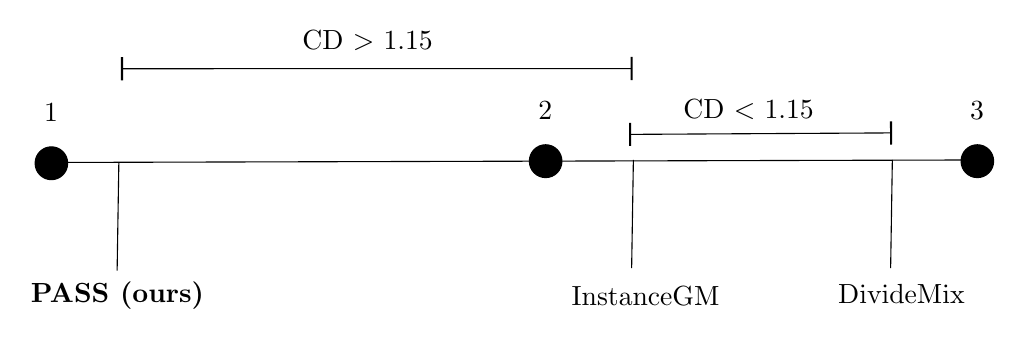
\begin{tikzpicture}[x=0.75pt,y=0.75pt,yscale=-1,xscale=1]
%uncomment if require: \path (0,404); %set diagram left start at 0, and has height of 404

%Straight Lines [id:da8701192106515236] 
\draw    (27.54,233.52) -- (463.44,232.34) ;
%Flowchart: Connector [id:dp14001705713759094] 
\draw  [fill={rgb, 255:red, 0; green, 0; blue, 0 }  ,fill opacity=1 ] (13.82,233.91) .. controls (13.82,229.54) and (17.33,226) .. (21.66,226) .. controls (25.99,226) and (29.5,229.54) .. (29.5,233.91) .. controls (29.5,238.28) and (25.99,241.82) .. (21.66,241.82) .. controls (17.33,241.82) and (13.82,238.28) .. (13.82,233.91) -- cycle ;
%Straight Lines [id:da13800813681196056] 
\draw    (54.16,233.52) -- (53.33,285.68) ;
%Straight Lines [id:da6386532806757288] 
\draw    (302.06,232.34) -- (301.22,284.49) ;
%Straight Lines [id:da9280208457661863] 
\draw    (426.83,232.34) -- (426,284.49) ;
%Straight Lines [id:da30121191187648466] 
\draw    (55.69,188.37) -- (301.21,188.29) ;
\draw [shift={(301.21,188.29)}, rotate = 179.98] [color={rgb, 255:red, 0; green, 0; blue, 0 }  ][line width=0.75]    (0,5.59) -- (0,-5.59)   ;
\draw [shift={(55.69,188.37)}, rotate = 179.98] [color={rgb, 255:red, 0; green, 0; blue, 0 }  ][line width=0.75]    (0,5.59) -- (0,-5.59)   ;
%Flowchart: Connector [id:dp051750127253487266] 
\draw  [fill={rgb, 255:red, 0; green, 0; blue, 0 }  ,fill opacity=1 ] (251.94,232.91) .. controls (251.94,228.54) and (255.45,225) .. (259.78,225) .. controls (264.12,225) and (267.63,228.54) .. (267.63,232.91) .. controls (267.63,237.28) and (264.12,240.82) .. (259.78,240.82) .. controls (255.45,240.82) and (251.94,237.28) .. (251.94,232.91) -- cycle ;
%Flowchart: Connector [id:dp17166445278398212] 
\draw  [fill={rgb, 255:red, 0; green, 0; blue, 0 }  ,fill opacity=1 ] (459.94,232.91) .. controls (459.94,228.54) and (463.45,225) .. (467.78,225) .. controls (472.12,225) and (475.63,228.54) .. (475.63,232.91) .. controls (475.63,237.28) and (472.12,240.82) .. (467.78,240.82) .. controls (463.45,240.82) and (459.94,237.28) .. (459.94,232.91) -- cycle ;
%Straight Lines [id:da36999664715996494] 
\draw    (300.5,220) -- (426.21,219.29) ;
\draw [shift={(426.21,219.29)}, rotate = 179.67] [color={rgb, 255:red, 0; green, 0; blue, 0 }  ][line width=0.75]    (0,5.59) -- (0,-5.59)   ;
\draw [shift={(300.5,220)}, rotate = 179.67] [color={rgb, 255:red, 0; green, 0; blue, 0 }  ][line width=0.75]    (0,5.59) -- (0,-5.59)   ;

% Text Node
\draw (16.87,204.09) node [anchor=north west][inner sep=0.75pt]   [align=left] {1};
% Text Node
\draw (10.5,289.62) node [anchor=north west][inner sep=0.75pt]   [align=left] {\textbf{PASS (ours)}};
% Text Node
\draw (271.05,291.99) node [anchor=north west][inner sep=0.75pt]   [align=left] {InstanceGM};
% Text Node
\draw (399.48,290.81) node [anchor=north west][inner sep=0.75pt]   [align=left] {DivideMix};
% Text Node
\draw (141.34,168.86) node [anchor=north west][inner sep=0.75pt]   [align=left] {CD $>$ 1.15};
% Text Node
\draw (255,203.09) node [anchor=north west][inner sep=0.75pt]   [align=left] {2};
% Text Node
\draw (463,203.09) node [anchor=north west][inner sep=0.75pt]   [align=left] {3};
% Text Node
\draw (324.91,202.02) node [anchor=north west][inner sep=0.75pt]   [align=left] {CD $<$ 1.15};


\end{tikzpicture}}
    \caption{Critical Difference (CD) diagram comparing DivideMix~\cite{li2020dividemix}, InstanceGM~\cite{Garg_2023_WACV}, and DivideMix-PASS (ours). Average ranks are derived from performance across datasets, with lines indicating the range of non-significant differences per the Nemenyi test. This test estimated the CD value of \(1.15\), which is used to estimate if two models are different with the significance level of \(0.1\). DivideMix-PASS demonstrates statistically significant superiority, InstanceGM~\cite{Garg_2023_WACV} and DivideMix~\cite{li2020dividemix} are not significantly different.}
    
    %\cuong{Is there a typo when placing DivideMix and InstanceGM since InstanceGM outperforms DivideMix in all the datasets used in this comparison?}\gustavo{I agree, it seems to have a typo there.}\arpit{Apologies, typo updated}
    
    % \cuong{Why is this figure changed compared to its previous version? Why is there a line connecting DivideMix and InstanceGM?}\gustavo{I agree with Cuong -- the figure that you showed in our last meeting should replace this one.}}
    \label{fig:stats_cd_diagram}
\end{figure}



To further understand these differences, we applied the post-hoc Nemenyi test. The test results showed significant differences between some of the methods. The Critical Difference (CD) value was calculated to be approximately \(1.15\). Based on this value, the methods whose average ranks differ by at least this CD value are considered significantly different at the \(0.1\) confidence level. Our analysis indicates that PASS is significantly different from both DivideMix and InstanceGM, as denoted by the Nemenyi test p-values (\(0.001\) against both). However, there is no significant difference between DivideMix and InstanceGM, as their comparison yields a p-value of \(0.109268\), which is above our threshold for significance. This comprehensive statistical analysis illustrates (\cref{fig:stats_cd_diagram}) the comparative effectiveness of these methods in handling various types and degrees of noise in datasets, affirming that DivideMix-PASS (ours) exhibits a statistically significant improvement over the other methods under study.



\subsection{Empirical Analysis on Sample Selection}\label{subsec:sample_selection}
% \cuong{Could we move this section into the ablation studies since it is slightly abrupt without properly introducing datasets, models and other settings.}
% \begin{figure}[t]
%     \centering
%     \begin{subfigure}[b]{0.3\textwidth}
%         \centering
%         \begin{tikzpicture}
%             \pgfplotstableread[col sep=comma, header=true]{csv/f1.tex} \myTable

%             \begin{axis}[
%                 height = 0.6\linewidth,
%                 width = 0.8\linewidth,
%                 xlabel={\textnumero~of epochs},
%                 xlabel style={font=\footnotesize},
%                 xticklabel style = {font=\footnotesize},
%                 xmin=40,
%                 xmax=310,
%                 ylabel={F1-score},
%                 ylabel style={font=\footnotesize, yshift=-0.5em},
%                 yticklabel style = {font=\footnotesize},
%                 scale only axis
%             ]
%                 \addplot[mark=none, MidnightBlue, thick, solid] table[x={epochs}, y={FINE}]{\myTable};
%                 \addplot[mark=none, BurntOrange, thick, densely dashed] table[x={epochs}, y={SmallLoss}]{\myTable};
%                 \addplot[mark=none, BrickRed, solid, thick, dashdotted] table[x={epochs}, y={PASS}]{\myTable};
%             \end{axis}
%         \end{tikzpicture}
%         \caption{F1 Score}
%         \label{fig:f1}
%     \end{subfigure}
%     \hfill
%     \begin{subfigure}[b]{0.3\textwidth}
%         \centering
%         \begin{tikzpicture}
%             \pgfplotstableread[col sep=comma, header=true]{csv/precision.tex} \myTable

%             \begin{axis}[
%                 height = 0.6\linewidth,
%                 width = 0.8\linewidth,
%                 xlabel={\textnumero~of epochs},
%                 xlabel style={font=\footnotesize},
%                 xticklabel style = {font=\footnotesize},
%                 xmin=40,
%                 xmax=310,
%                 ylabel={Precision},
%                 ylabel style={font=\footnotesize, yshift=-0.5em},
%                 yticklabel style = {font=\footnotesize},
%                 legend entries={FINE, Small loss, PASS},
%                 legend style={draw=none, font=\tiny, /tikz/every even column/.append style={column sep=1em}},
%                 legend image post style={scale=.75},
%                 legend columns=2,
%                 legend cell align={right},
%                 legend pos=north east,
%                 scale only axis
%             ]
%                 \addplot[mark=none, MidnightBlue, thick, solid] table[x={epochs}, y={FINE}]{\myTable};
%                 \addplot[mark=none, BurntOrange, thick, densely dashed] table[x={epochs}, y={SmallLoss}]{\myTable};
%                 \addplot[mark=none, BrickRed, solid, thick, dashdotted] table[x={epochs}, y={PASS}]{\myTable};
%             \end{axis}
%         \end{tikzpicture}
%         \caption{Precision}
%         \label{fig:precision}
%     \end{subfigure}
%     % \vspace{1em}
%     \begin{subfigure}[b]{0.3\textwidth}
%         \centering
%         \begin{tikzpicture}
%             \pgfplotstableread[col sep=comma, header=true]{csv/clean.tex} \myTable

%             \begin{axis}[
%                 height = 0.6\linewidth,
%                 width = 0.8\linewidth,
%                 xlabel={\textnumero~of epochs},
%                 xlabel style={font=\font=\tiny},
%                 xticklabel style = {font=\font=\tiny},
%                 xmin=40,
%                 xmax=310,
%                 ylabel={Ratio of clean data},
%                 ylabel style={font=\font=\tiny, yshift=-0.5em},
%                 yticklabel style = {font=\tiny},
%                 % legend entries={FINE, Small loss, PASS},
%                 % legend style={draw=none, font=\tiny, /tikz/every even column/.append style={column sep=1em}},
%                 % legend image post style={scale=.75},
%                 % legend columns=2,
%                 % legend cell align={right},
%                 % legend pos=north east,
%                 scale only axis
%             ]
%                 \addplot[mark=none, MidnightBlue, thick, solid] table[x={epochs}, y={FINE}]{\myTable};
%                 \addplot[mark=none, BurntOrange, thick, densely dashed] table[x={epochs}, y={SmallLoss}]{\myTable};
%                 \addplot[mark=none, BrickRed, solid, thick, dashdotted] table[x={epochs}, y={PASS}]{\myTable};

%                 % plot the ideal noise ratio
%                 \addplot[mark=none, style={densely dashed}] coordinates {
%                     (50, 0.5)
%                     (300, 0.5)
%                 };
%                 \node[above, color=Black, rotate=0, ] at (100, 0.5) {\tiny{ideal ratio}};
%             \end{axis}
%         \end{tikzpicture}
%         \caption{Ratio of data classified as clean}
%         \label{fig:ratio}
%     \end{subfigure}
%     \caption{Comparative analysis of the effectiveness of selecting clean or noisy samples, with reference to three metrics: (a) F1-score, (b) precision, and (c) ratio of data classified as clean. The comparison is made between PASS (red), the small-loss approach~\cite{jiang2018mentornet} (yellow), and feature-based selection~\cite{kim2021fine} (blue) (all are based on DivideMix backbone~\cite{li2020dividemix}), implemented on the CIFAR-100 dataset\cite{krizhevsky2009learning} at \(0.5\) IDN noise rate, as described in~\cite{xia2020part}.}
%     \label{fig:empirical_graph}
% \end{figure}

\begin{figure*}[t]
    \centering
    \hspace{-1em}
    \begin{subfigure}[b]{0.3\textwidth}
        \centering
        \begin{tikzpicture}
            \pgfplotstableread[col sep=comma, header=true]{csv/f1.tex} \myTable

            \begin{axis}[
                height = 0.6\linewidth,
                width = 0.8\linewidth,
                xlabel={\textnumero~of epochs},
                xlabel style={font=\scriptsize},
                xticklabel style = {font=\scriptsize},
                xmin=40,
                xmax=310,
                ylabel={F1-score},
                ylabel style={font=\scriptsize, yshift=-0.5em},
                yticklabel style = {font=\scriptsize},
                scale only axis
            ]
                \addplot[mark=none, MidnightBlue, thick, solid] table[x={epochs}, y={FINE}]{\myTable};
                \addplot[mark=none, BurntOrange, thick, densely dashed] table[x={epochs}, y={SmallLoss}]{\myTable};
                \addplot[mark=none, BrickRed, solid, thick, dashdotted] table[x={epochs}, y={PASS}]{\myTable};
            \end{axis}
        \end{tikzpicture}
        \caption{F1 Score}
        \label{fig:f1}
    \end{subfigure}
    \hfill
    \begin{subfigure}[b]{0.3\textwidth}
        \centering
        \begin{tikzpicture}
            \pgfplotstableread[col sep=comma, header=true]{csv/precision.tex} \myTable

            \begin{axis}[
                height = 0.6\linewidth,
                width = 0.8\linewidth,
                xlabel={\textnumero~of epochs},
                xlabel style={font=\scriptsize},
                xticklabel style = {font=\scriptsize},
                xmin=40,
                xmax=310,
                ylabel={Precision},
                ylabel style={font=\scriptsize, yshift=-0.5em},
                yticklabel style = {font=\scriptsize},
                legend entries={FINE, Small loss, PASS},
                legend style={draw=none, font=\tiny, /tikz/every even column/.append style={column sep=0.1em}},
                legend image post style={scale=.75},
                legend columns=2,
                legend cell align={left},
                % legend pos= north east,
                legend style={at={(0.0,0.6)},anchor=west},
                scale only axis
            ]
                \addplot[mark=none, MidnightBlue, thick, solid] table[x={epochs}, y={FINE}]{\myTable};
                \addplot[mark=none, BurntOrange, thick, densely dashed] table[x={epochs}, y={SmallLoss}]{\myTable};
                \addplot[mark=none, BrickRed, solid, thick, dashdotted] table[x={epochs}, y={PASS}]{\myTable};
            \end{axis}
        \end{tikzpicture}
        \caption{Precision}
        \label{fig:precision}
    \end{subfigure}
    \hfill
    \begin{subfigure}[b]{0.35\textwidth}
        \centering
        \begin{tikzpicture}
            \pgfplotstableread[col sep=comma, header=true]{csv/clean.tex} \myTable

            \begin{axis}[
                height = 0.514\linewidth,
                width = 0.686\linewidth,
                xlabel={\textnumero~of epochs},
                xlabel style={font=\scriptsize},
                xticklabel style = {font=\scriptsize},
                xmin=40,
                xmax=310,
                ylabel={Ratio of clean data},
                ylabel style={font=\scriptsize, yshift=-0.5em},
                yticklabel style = {font=\scriptsize},
                scale only axis
            ]
                \addplot[mark=none, MidnightBlue, thick, solid] table[x={epochs}, y={FINE}]{\myTable};
                \addplot[mark=none, BurntOrange, thick, densely dashed] table[x={epochs}, y={SmallLoss}]{\myTable};
                \addplot[mark=none, BrickRed, solid, thick, dashdotted] table[x={epochs}, y={PASS}]{\myTable};

                % plot the ideal noise ratio
                \addplot[mark=none, style={densely dashed}] coordinates {
                    (50, 0.5)
                    (300, 0.5)
                };
                \node[above, color=Black, rotate=0, ] at (110, 0.5) {\scriptsize{ideal ratio}};
            \end{axis}
        \end{tikzpicture}
        \caption{Ratio of data classified as clean}
        \label{fig:ratio}
    \end{subfigure}
    \caption{Comparative analysis of the effectiveness of selecting clean or noisy samples, with reference to three metrics: (a) F1-score, (b) precision, and (c) ratio of data classified as clean. The comparison is made between PASS (dash-dot red), the small-loss approach~\cite{jiang2018mentornet} (dashed yellow), and feature-based selection FINE~\cite{kim2021fine} (solid blue) (all are based on DivideMix backbone~\cite{li2020dividemix}), implemented on the CIFAR-100 dataset\cite{krizhevsky2009learning} at \(0.5\) IDN noise rate, as described in~\cite{xia2020part}. }
    \label{fig:empirical_graph}
\end{figure*}

In this section, we conduct an empirical analysis of the PASS algorithm. Detailed in \cref{subsec:empirical_subsec_cifar}, the analysis compares the effectiveness of PASS against small loss~\cite{li2020dividemix} and FINE~\cite{kim2021fine} approaches on the CIFAR100~\cite{krizhevsky2009learning}, specifically at \(0.5, 0.4, \text{ and } 0.2\) IDN~\cite{xia2020part}. The comparison focuses on metrics F1 score, precision, and the ratio of clean samples, employing DivideMix~\cite{li2020dividemix} as the base model for PASS. Similarly,~\cref{subsec:empirical_subsec_clothing} extends this analysis to the Clothing1M~\cite{xiao2015learning}, a real-world dataset. Here, the comparison is between AugDesc~\cite{nishi2021augmentation}, and PASS with baseline AugDesc~\cite{nishi2021augmentation}.

\subsubsection{Analysis of PASS Performance at Various Noise Rates on CIFAR100}\label{subsec:empirical_subsec_cifar}
\paragraph{IDN setting at high noise rate (e.g., 50\%)} To empirically analyse PASS, we focus on the challenging IDN synthetic noise at \(50\%\) noise rate~\cite{xia2020part} on CIFAR-100~\cite{krizhevsky2009learning}.
\cref{fig:empirical_graph} shows three graphs to measure the performance of the clean sample classification, namely: \cref{fig:f1} shows \emph{F1 score}, \cref{fig:precision} shows \emph{precision}, and \cref{fig:ratio} shows the \emph{ratio of the data classified as clean}.
We use these graphs to compare our PASS against the small-loss hypothesis~\cite{li2020dividemix}, and feature-based approach~\cite{kim2021fine} (all using DivideMix~\cite{li2020dividemix} as the robust noisy-label training algorithm). We have only considered the methods of sample selection and have not incorporated the methods that involve sample relabeling within this analysis~\cite{feng2021ssr}. 
% \gustavo{please add citation to a sample relabeling method}.

\cref{fig:ratio} shows the proportion of data classified as clean (by the model). 
It is evident that the small-loss~\cite{li2020dividemix} hypothesis and the feature-based approach~\cite{kim2021fine} consistently yield a ratio of around $0.70 - 0.65$ during the training process, while our approach maintains a ratio of around $0.50-0.45$. 
As we know from the setup, the optimal rate (ideal ratio) should be $\approx$ $0.50$. This indicates that our approach is more capable of identifying the correct proportion of noisy-label samples for the IDN at \(50\%\) on CIFAR-100. 
However, that proportion alone does not ensure that clean samples are accurately selected. 
Therefore, we also calculated the F1 score (\cref{fig:f1}) and the precision (\cref{fig:precision}), both of which show superior results using our approach. 
More specifically, \cref{fig:f1} shows that our strategy exhibits a consistently higher F1 score compared to other approaches, achieving the final result of $0.87$, which is better than other approaches, such as small-loss and feature-based~\cite{kim2021fine} that present a similar result of $0.75$. Another important comparison measure is precision. PASS shows very high precisions of more than $0.96$, while small-loss~\cite{li2020dividemix} and feature-based~\cite{kim2021fine} show much lower precision values around $0.72$. This empirical analysis suggests that our method is more efficacious at correctly identifying positive and negative samples from the training set than other competing approaches.

\paragraph{IDN settings at low and intermediate noise rates} (e.g., \(20\% \text{ and } 40\%\)) We further extended our empirical analysis to include other challenging IDN noise cases~\cite{xia2020part} at rates of $40\%$ and $20\%$, as shown in \cref{fig:0.4_supp,fig:0.2_supp} on CIFAR-100~\cite{krizhevsky2009learning} respectively. These plots compare our PASS (using DivideMix~\cite{li2020dividemix}) against the small-loss~\cite{li2020dividemix} and feature-based~\cite{kim2021fine} approaches by measuring the 
classification performance of clean samples based on (a) F1 score, (b) precision, and (c) ratio of data classified as clean. 

\begin{figure*}[t]
    \centering
    \begin{subfigure}[b]{0.3\textwidth}
        \centering
        \begin{tikzpicture}
            \pgfplotstableread[col sep=comma, header=true]{supp_cifar0.4_csv/f1.tex} \myTable
            \begin{axis}[
                height = 0.6\linewidth,
                width = 0.8\linewidth,
                xlabel={\textnumero~of epochs},
                xlabel style={font=\scriptsize},
                xticklabel style = {font=\scriptsize},
                ylabel={F1-score},
                ylabel style={font=\scriptsize, yshift=-0.5em},
                yticklabel style = {font=\scriptsize},
                scale only axis
            ]
                \addplot[mark=none, MidnightBlue, thick, solid] table[x={epochs}, y={FINE}]{\myTable};
                \addplot[mark=none, BurntOrange, thick, densely dashed] table[x={epochs}, y={SmallLoss}]{\myTable};
                \addplot[mark=none, BrickRed, solid, thick, dashdotted] table[x={epochs}, y={PASS}]{\myTable};
            \end{axis}
        \end{tikzpicture}
        \caption{F1 Score}
        \label{fig:0.4_f1}
    \end{subfigure}
    \hfill
    \begin{subfigure}[b]{0.3\textwidth}
        \centering
        \begin{tikzpicture}
            \pgfplotstableread[col sep=comma, header=true]{supp_cifar0.4_csv/precision.tex} \myTable
            \begin{axis}[
                height = 0.6\linewidth,
                width = 0.8\linewidth,
                xlabel={\textnumero~of epochs},
                xlabel style={font=\scriptsize},
                xticklabel style = {font=\scriptsize},
                ylabel={Precision},
                ylabel style={font=\scriptsize, yshift=-0.5em},
                yticklabel style = {font=\scriptsize},
                scale only axis
            ]
                \addplot[mark=none, MidnightBlue, thick, solid] table[x={epochs}, y={FINE}]{\myTable};
                \addplot[mark=none, BurntOrange, thick, densely dashed] table[x={epochs}, y={SmallLoss}]{\myTable};
                \addplot[mark=none, BrickRed, solid, thick, dashdotted] table[x={epochs}, y={PASS}]{\myTable};
            \end{axis}
        \end{tikzpicture}
        \caption{Precision}
        \label{fig:0.4_precision}
    \end{subfigure}
    \hfill
    \begin{subfigure}[b]{0.3\textwidth}
        \centering
        \begin{tikzpicture}
            \pgfplotstableread[col sep=comma, header=true]{supp_cifar0.4_csv/clean.tex} \myTable

            \begin{axis}[
                height = 0.6\linewidth,
                width = 0.8\linewidth,
                xlabel={\textnumero~of epochs},
                xlabel style={font=\scriptsize},
                xticklabel style = {font=\scriptsize},
                ylabel={Ratio of clean data},
                ylabel style={font=\scriptsize, yshift=-0.5em},
                yticklabel style = {font=\scriptsize},
                legend entries={FINE, Small loss, PASS},
                legend style={draw=none, font=\scriptsize},
                legend image post style={scale=1.},
                legend cell align={left},
                legend pos=north east,
                scale only axis
            ]
                \addplot[mark=none, MidnightBlue, thick, solid] table[x={epochs}, y={FINE}]{\myTable};
                \addplot[mark=none, BurntOrange, thick, densely dashed] table[x={epochs}, y={SmallLoss}]{\myTable};
                \addplot[mark=none, BrickRed, solid, thick, dashdotted] table[x={epochs}, y={PASS}]{\myTable};

                % plot the ideal noise ratio
                \addplot[mark=none, style={densely dashed}] coordinates {
                    (50, 0.6)
                    (300, 0.6)
                };
                \node[below, color=Black, rotate=0, ] at (95, 0.6) {\scriptsize{ideal ratio}};
            \end{axis}
        \end{tikzpicture}
        \caption{Ratio of clean classified data}
        
        \label{fig:0.4_clean}
    \end{subfigure}
    \caption{Graphs to compare the effectiveness of selecting clean or noisy samples, regarding three metrics: (a) F1-score, (b) precision, and (c) ratio of data classified as clean. The comparison is made between our PASS (dash-dot \textcolor{BrickRed}{red}), small-loss approach~\cite{jiang2018mentornet} (dashed \textcolor{BurntOrange}{yellow}),  and feature-based approach FINE~\cite{kim2021fine} (solid \textcolor{MidnightBlue}{blue}) (all on base model DivideMix~\cite{li2020dividemix}), implemented on the CIFAR-100 dataset\cite{krizhevsky2009learning} at \(0.4\) IDN noise rate, as described in~\cite{xia2020part}.}\label{fig:0.4_supp}
\end{figure*}

\begin{figure*}[t]
    \begin{subfigure}[b]{0.3\textwidth}
        \centering
        \begin{tikzpicture}
            \pgfplotstableread[col sep=comma, header=true]{supp_cifar0.2_csv/f1.tex} \myTable
            \begin{axis}[
                height = 0.6\linewidth,
                width = 0.8\linewidth,
                xlabel={\textnumero~of epochs},
                xlabel style={font=\scriptsize},
                xticklabel style = {font=\scriptsize},
                ylabel={F1-score},
                ylabel style={font=\scriptsize, yshift=-0.5em},
                yticklabel style = {font=\scriptsize},
                scale only axis
            ]
                \addplot[mark=none, MidnightBlue, thick, solid] table[x={epochs}, y={FINE}]{\myTable};
                \addplot[mark=none, BurntOrange, thick, densely dashed] table[x={epochs}, y={SmallLoss}]{\myTable};
                \addplot[mark=none, BrickRed, solid, thick, dashdotted] table[x={epochs}, y={PASS}]{\myTable};
            \end{axis}
        \end{tikzpicture}
        \caption{F1 Score}
        \label{fig:0.2_f1}
    \end{subfigure}
    \hfill
    \begin{subfigure}[b]{0.3\textwidth}
        \centering
        \begin{tikzpicture}
            \pgfplotstableread[col sep=comma, header=true]{supp_cifar0.2_csv/precision.tex} \myTable
            \begin{axis}[
                height = 0.6\linewidth,
                width = 0.8\linewidth,
                xlabel={\textnumero~of epochs},
                xlabel style={font=\scriptsize},
                xticklabel style = {font=\scriptsize},
                ylabel={Precision},
                ylabel style={font=\scriptsize, yshift=-0.5em},
                yticklabel style = {font=\scriptsize},
                legend entries={FINE, Small loss, PASS},
                legend style={draw=none, font=\scriptsize},
                legend image post style={scale=1.},
                legend cell align={left},
                legend pos=south east,
                scale only axis
            ]
                \addplot[mark=none, MidnightBlue, thick, solid] table[x={epochs}, y={FINE}]{\myTable};
                \addplot[mark=none, BurntOrange, thick, densely dashed] table[x={epochs}, y={SmallLoss}]{\myTable};
                \addplot[mark=none, BrickRed, solid, thick, dashdotted] table[x={epochs}, y={PASS}]{\myTable};
            \end{axis}
        \end{tikzpicture}
        \caption{Precision}
        \label{fig:0.2_precision}
    \end{subfigure}
    \hfill
    \begin{subfigure}[b]{0.3\textwidth}
        \centering
        \begin{tikzpicture}
            \pgfplotstableread[col sep=comma, header=true]{supp_cifar0.2_csv/clean.tex} \myTable
            \begin{axis}[
                height = 0.6\linewidth,
                width = 0.8\linewidth,
                xlabel={\textnumero~of epochs},
                xlabel style={font=\scriptsize},
                xticklabel style = {font=\scriptsize},
                ylabel={Ratio of clean data},
                ylabel style={font=\scriptsize, yshift=-0.5em},
                yticklabel style = {font=\scriptsize},
                % legend entries={FINE, Small loss, PASS},
                % legend style={draw=none, font=\scriptsize},
                % legend image post style={scale=1.},
                % legend cell align={left},
                % legend pos=south east,
                scale only axis
            ]
                \addplot[mark=none, MidnightBlue, thick, solid] table[x={epochs}, y={FINE}]{\myTable};
                \addplot[mark=none, BurntOrange, thick, densely dashed] table[x={epochs}, y={SmallLoss}]{\myTable};
                \addplot[mark=none, BrickRed, solid, thick, dashdotted] table[x={epochs}, y={PASS}]{\myTable};

                % plot the ideal noise ratio
                \addplot[mark=none, style={densely dashed}] coordinates {
                    (50, 0.8)
                    (300, 0.8)
                };
                \node[above, color=Black, rotate=0, ] at (120, 0.8) {\scriptsize{ideal ratio}};
            \end{axis}
        \end{tikzpicture}
        \caption{Ratio of clean classified data}
        \label{fig:0.2_clean}
    \end{subfigure}
    \caption{Graphs to compare the effectiveness of selecting clean or noisy samples, regarding three metrics: (a) F1-score, (b) precision, and (c) ratio of data classified as clean. The comparison is made between our PASS (dash-dot \textcolor{BrickRed}{red}), small-loss approach~\cite{jiang2018mentornet} (dashed \textcolor{BurntOrange}{yellow}), and feature-based approach FINE~\cite{kim2021fine} (solid \textcolor{MidnightBlue}{blue}) (all on base model DivideMix~\cite{li2020dividemix}), implemented on the CIFAR-100 dataset\cite{krizhevsky2009learning} at \(0.2\) IDN noise rate, as described in~\cite{xia2020part}.}\label{fig:0.2_supp}
\end{figure*}

 From \cref{fig:0.4_supp,fig:0.2_supp}, it is clear that as training evolves, PASS gets closer to the ideal proportion of clean-label samples available for training than the small-loss~\cite{li2020dividemix} and feature-based~\cite{kim2021fine} approaches, suggesting that our approach
is more capable of identifying the correct proportion of noisy-label samples for the IDN noise. 
This proportion alone does not imply accuracy. Therefore, we also provide graphs with F1 and precision scores, which help to highlight the advantages of using our peer agreement for sample selection. 
More specifically, \cref{fig:0.4_supp,fig:0.2_supp} show that our strategy exhibits a consistently superior F1 score compared to other approaches for noise rates $40\%$ (\cref{fig:0.4_f1}) and $20\%$ (\cref{fig:0.2_f1}). PASS achieves a final result of $0.92$, which directly reflects the improvement in the performance of PASS when compared to small-loss~\cite{li2020dividemix} and feature-based~\cite{kim2021fine} with similar results of $0.8-0.85$ at noise rate $40\%$. Whilst feature-based~\cite{kim2021fine} and PASS are very competitive in F1 score for noise rate $20\%$ with a value around $0.94$, small-loss~\cite{li2020dividemix} stays around $0.89$.
PASS shows an outstanding precision higher than $0.98$, while small-loss~\cite{li2020dividemix} and feature-based~\cite{kim2021fine} show much smaller precision values of around $0.8$ for noise rate $40\%$ (\cref{fig:0.4_precision}). Moreover, all methods are very competitive in precision at a low noise rate of $20\%$ (\cref{fig:0.2_precision}). Our empirical analysis shows that our method outperforms other competing approaches in correctly identifying positive and negative samples from the training set across all noise levels.


\subsubsection{Empirical Insights on PASS using Clothing1M}\label{subsec:empirical_subsec_clothing}

Although Clothing1M~\cite{xiao2015learning} offers a clean validation set, we did not incorporate it into our training process. However, we used this clean validation set to assess and compare the effectiveness of PASS and baseline AugDesc~\cite{nishi2021augmentation}. For AugDesc training with and without PASS, we have used the \emph{DM-AugDesc-WS-WAW} version of training, as mentioned in AugDesc~\cite{nishi2021augmentation}. As mentioned in \cref{table:clothing1M},  
%\rafa{This refernce is broken in the text -> }~\cref{table:Clothing1M} 
our results are competitive with the existing model. Although both baseline methods are competitive, PASS is still capable of outperforming based on: (\subref{fig:cloth_f1}) F1, (\subref{fig:cloth_precision}) precision, and (\subref{fig:cloth_ratio}) the ratio of clean data in \cref{fig:clothing_supp}.

\begin{figure*}[t!]
    \centering
    \begin{subfigure}[b]{0.3\textwidth}
        \centering
        \begin{tikzpicture}
            \pgfplotstableread[col sep=comma, header=true]{clothing1m_csv/f1.tex} \myTable
            \begin{axis}[
                height = 0.6\linewidth,
                width = 0.8\linewidth,
                xlabel={\textnumero~of epochs},
                xlabel style={font=\scriptsize},
                xticklabel style = {font=\scriptsize},
                ylabel={F1-score},
                ylabel style={font=\scriptsize, yshift=-0.5em},
                yticklabel style = {font=\scriptsize},
                legend entries={AugDesc, AugDesc-PASS},
                legend style={draw=none, font=\scriptsize},
                legend image post style={scale=0.5},
                legend cell align={left},
                legend pos=south east,
                scale only axis
            ]
                \addplot[mark=none, BurntOrange, thick, densely dashed] table[x={epochs}, y={SmallLoss}]{\myTable};
                \addplot[mark=none, MidnightBlue, solid, thick, solid] table[x={epochs}, y={PASS}]{\myTable};
            \end{axis}
        \end{tikzpicture}
        \caption{F1 Score}
        \label{fig:cloth_f1}
    \end{subfigure}
    \hfill
    \begin{subfigure}[b]{0.3\textwidth}
        \centering

        \begin{tikzpicture}
            \pgfplotstableread[col sep=comma, header=true]{clothing1m_csv/precision_.tex} \myTable

            \begin{axis}[
                height = 0.6\linewidth,
                width = 0.8\linewidth,
                xlabel={\textnumero~of epochs},
                xlabel style={font=\scriptsize},
                xticklabel style = {font=\scriptsize},
                ylabel={Precision},
                ylabel style={font=\scriptsize, yshift=-0.5em},
                yticklabel style = {font=\scriptsize},
                scale only axis
            ]
                \addplot[mark=none, BurntOrange, thick, densely dashed] table[x={epochs}, y={SmallLoss}]{\myTable};
                \addplot[mark=none, MidnightBlue, solid, thick, solid] table[x={epochs}, y={PASS}]{\myTable};
            \end{axis}
        \end{tikzpicture}
        \caption{Precision}
        \label{fig:cloth_precision}
    \end{subfigure}
    \hfill
    \begin{subfigure}[b]{0.3\textwidth}
        \centering

        \begin{tikzpicture}
            \pgfplotstableread[col sep=comma, header=true]{clothing1m_csv/clean.tex} \myTable
            \begin{axis}[
                height = 0.6\linewidth,
                width = 0.8\linewidth,
                xlabel={\textnumero~of epochs},
                xlabel style={font=\scriptsize},
                xticklabel style = {font=\scriptsize},
                ylabel={Ratio of clean data},
                ylabel style={font=\scriptsize, yshift=-0.5em},
                yticklabel style = {font=\scriptsize},
                scale only axis
            ]
                \addplot[mark=none, BurntOrange, thick, densely dashed] table[x={epochs}, y={SmallLoss}]{\myTable};
                \addplot[mark=none, MidnightBlue, solid, thick, solid] table[x={epochs}, y={PASS}]{\myTable};
            \end{axis}
        \end{tikzpicture}
        \caption{Ratio of clean classified data}
        \label{fig:cloth_ratio}
    \end{subfigure}
    \caption{Graphs to compare the effectiveness of selecting clean or noisy samples, regarding three metrics: (a) F1-score, (b) precision, and (c) ratio of data classified as clean.
    The comparison is made between our approach AugDesc-PASS (solid \textcolor{MidnightBlue}{blue}) with baseline AugDesc approach~\cite{nishi2021augmentation} (dashed \textcolor{BurntOrange}{yellow}) on Clothing1M. We have used DM-AugDesc-WS-WAW version of training as mentioned in AugDesc~\cite{nishi2021augmentation}.}\label{fig:clothing_supp}
\end{figure*}